%!TEX program = xelatex

% 纸张模式:护眼模式-geye 朦胧模式-hazy
% 纸张尺寸:pad kindle pc normal screen
\documentclass[cn, blue, normal, 12pt]{elegantnote}

\title{数字图像处理与计算机视觉复习笔记}
\author{Xiaohei}
\version{0.1}
\date{\zhtoday}

\usepackage{pgfplots}
\pgfplotsset{compat=newest}
\usetikzlibrary{plotmarks}
\usetikzlibrary{arrows.meta}
\usepgfplotslibrary{patchplots}
\usepackage{grffile}
\usepackage{amsmath}
\usepackage{multirow}
\usepackage{bm}

\begin{document}

\setlength{\lineskip}{0}
\setlength{\parskip}{0}

\maketitle

\section{绪论}

\subsection{图像的基本概念}

\subsubsection{图像的概念}

\textbf{图像}是用各种观测系统以不同形式和手段观测客观世界而获得的,可以直接或间接作用于人眼并进而产生视知觉的实体。

\subsubsection{数字图像的概念}

把连续的图像$f(x,y)$在$2-D$空间$XY$和性质空间$F$都\textbf{离散化},这种离散化了的图像叫做\textbf{数字图像}。数字图像可以用$I(r,c)$来表示。

\subsubsection{图像的表达}

图像可以用\textbf{矩阵}或\textbf{矢量}表示。

图像的显示方式:\textbf{点方式}、\textbf{块方式}和\textbf{值方式}。

\subsection{图像处理技术分类}

\textbf{模拟图像处理}:包括光学处理和电子处理。速度快、可并行处理,但精度较差,灵活性差,很难有判断能力和非线性处理能力。

\textbf{数字图像处理}:用计算机处理或实时的硬件处理,也称计算机图像处理。处理精度高,处理内容丰富,可进行复杂的非线性处理,但处理速度还有待提高,分辨率及精度尚有一定限制。

\subsection{数字图像处理}

\textbf{数字图像处理的特点}:

\begin{enumerate}
    \item 图像信息量大、数据量也大。
    \item 图像处理技术综合性强。
    \item 图像信息理论与通信理论密切相关。
\end{enumerate}

\textbf{数字图像处理的方法}:

\begin{enumerate}
    \item 空域法:把图像看作是空间域平面中各个像素组成的集合,直接对二维函数进行相应处理。主要分为点处理法和邻域处理法。
    \item 频域法:先将图像从空域正变换到频域,在频域对图像进行处理,再反变换到空间域,得到处理结果。包括滤波、数据压缩、特征提取等。
\end{enumerate}

\textbf{数字图像处理系统的主要模块}:

\begin{enumerate}
    \item 图像信息的采集、存储、通信、显示;
    \item 数字图像的处理。
\end{enumerate}

\subsubsection{数字图像处理的发展方向}

\textbf{数字图像处理领域中需要进一步研究的问题}:

\begin{enumerate}
    \item 提高精度的同时还要解决处理速度的问题;
    \item 加强软件研究,创造新的处理方法;
    \item 加强边缘学科的研究工作,促进图像处理技术的发展;
    \item 加强理论研究,逐步形成图像处理科学自身的理论体系;
    \item 建立图像信息库和标准子程序,统一存放格式和检索,方便不同领域的图像交流和使用,实现资源共享。
\end{enumerate}

\textbf{数字图像处理技术未来的发展方向}:

\begin{enumerate}
    \item 围绕高清晰度电视(HDTV)的研制;
    \item 开展实时图像处理的理论及技术研究,向着高速化、高分辨率、立体化、多媒体化、智能化和标准化方向发展。
    \item 图像与图形相结合,朝着三维成像或多维成像的方向发展;
    \item 硬件芯片研究,把图像处理的众多功能固化在芯片上,更便于应用;
    \item 新理论和新算法研究。
\end{enumerate}

\section{图像与视觉系统}

\subsection{视觉过程}

视觉过程由光学过程、化学过程和神经处理过程顺序构成。

\subsubsection{光学过程}

光学过程:视觉过程从光源发光开始,光线被场景中的物体反射进入作为视觉感受器官人的左右眼睛,并在视网膜成像。

物体在视网膜上成像尺寸的计算:

\begin{equation}
    \frac{h}{l}=\frac{x}{L}
\end{equation}

其中$h$为物体的高度,$l$为物体距离观察者的距离,$L$为晶状体聚焦中心和视网膜间的距离,$x$为物体在视网膜上的成像尺寸。

$l>3m$时,晶状体具有最小的屈光能力,取$L=17mm$,$l<3m$时,晶状体具有最大的屈光能力,取$L=14mm$。

\subsubsection{化学过程}

化学过程:物体在视网膜上成像并引起视感觉,视感觉本质上是从分子的观点来理解光反应的基本性质(如亮度、颜色)。

视网膜表面分布有光接受细胞,分为两类:锥细胞:数量少,分辨率较高,对颜色很敏感。锥细胞视觉称为适亮视觉;柱细胞:数量多,分辨率较低,不感受颜色。柱细胞视觉称为适暗视觉。

\subsubsection{神经处理过程}

神经处理过程:光刺激在视网膜上经神经处理产生神经冲动,神经冲动沿视神经纤维传出眼睛,通过视觉通道传到大脑皮层,并引起视知觉,视知觉本质上体现神经系统接受视觉刺激后如何反应及其反应方式。

\subsection{光度学基本原理}

\subsubsection{点光源}

当光源的强度足够小,或距离观察者足够远,以至于眼睛无法分辨其形状时,可称为点光源。

在光度学中,光通量$\varPhi$用来表示光辐射的功率或光辐射量,单位是$\mathrm{lm}$(流明)。

立体角:从一点(称为立体角的顶点)出发通过一条闭合曲线上所有点的射线围成的空间部分,表示由顶点看闭合曲线时的视角。

立体角数值上等于以顶点为球心所作的球面上截出的部分面积与球面半径的平方之比,单位是$\mathrm{sr}$(球面度)。

\begin{equation}
    \varOmega=\frac{A}{r^2}
\end{equation}

其中$\varOmega$为立体角,$A$为以立体角的顶点为球心所作的球面上截出的部分面积,$r$为球面半径。

点光源$Q$沿某个方向$r$的发光强度$I$定义为沿此方向上单位立体角内发出的光通量。发光强度$I$单位:$\mathrm{cd}$(坎[德拉])。

\begin{equation}
    I=\frac{\varPhi}{\varOmega}=\frac{\varPhi}{4\pi r^2/r^2}=\frac{\varPhi}{4\pi}
\end{equation}

\subsubsection{扩展光源}

实际中的光源总有一定的发光面积,称为扩展光源。

扩展光源表面的每块面元$\mathrm{d}S$沿某个方向$r$有一定的发光强度$I$,扩展光源在沿$r$方向的总发光强度为各个面元沿$r$方向的发光强度之和。

\subsubsection{亮度}

面元$\mathrm{d}S$沿$r$方向的亮度$B$定义为在$r$方向上单位投影面积的发光强度。亮度$B$的单位:$\mathrm{cd/m^2}$(坎[德拉]每平方米)。

\begin{equation}
    B=\frac{I}{S'}=\frac{I}{S\cos{\theta}}=\frac{\varPhi}{\varOmega S\cos{\theta}}
\end{equation}

其中$\theta$为$r$与$S$的法线$N$的夹角。

\subsubsection{主观亮度}

人的视觉系统感受到的物体的亮度称为主观亮度。主观亮度受到物体表面与周围环境亮度之间相对关系的影响。

同时对比度表明人眼对某个区域感受到的主观亮度并不仅仅依赖于该区域本身的亮度,反射相同亮度的物体放在较暗的背景里会显得比较亮。

马赫带效应是指人类视觉系统有趋向于过高或过低估计不同亮度区域边界值的现象。

\subsubsection{照度}

照度定义为照射在物体单位面积上的光通量。从辐射学的角度也称辐照度,表示单位面积的入射功率。记为$E$,单位是$\mathrm{lx}$(勒[克斯])。

\begin{equation}
    E=\frac{\varPhi}{S}
\end{equation}

\subsection{采样和量化}

一副连续图像$f(x,y)$必须在空间和幅度上都离散化后才能被计算机处理。其空间坐标的离散化叫做空间采样(简称采样),确定图像的空间分辨率。灰度值的离散化叫做灰度量化(简称量化),确定图像的幅度分辨率。

如果一副图像的尺寸(空间分辨率)为$M\times N$,则表明在成像时采了$M\times N$个样,图像包含$M\times N$个像素。如果对每个像素都用$G$个灰度值中的一个来赋值,则表明在成像时量化成了$G$个灰度级(幅度分辨率)。

一般将这些量均取为$2$的整数次幂。若$L=2^k$,则图像所需比特数$b=M\times N\times k$。

PAL制式的图像传输速率为25帧/秒。

\subsection{图像类型}

颜色深度:每一个像素的颜色值所占的二进制位数。

颜色数:每一个像素所有可能的颜色值的个数。

二值图像:也称单色图像或1位图像,即颜色深度为1的图像。一般地,0表示黑,1表示白。

灰度图像:每个像素由8位组成,其值范围为$0\sim 255$,表示256种不同的灰度级。存储文件包含图像颜色表,其RGB分量的值相等。

真彩色图像:每个像素由RGB三个分量组成,每个分量各占8位,每个像素共占24位。RGB每个分量的取值范围为$0\sim 255$,图像文件中不包含图像颜色表。

伪彩色图像:存储文件包含图像颜色表,其RGB分量的值不全相等。分为256色彩色图像(8位)、16色彩色图像(4位)。

\section{像素空间关系}

\subsection{像素间的基本关系}

\subsubsection{像素的邻域}

一个像素的邻近像素组成该像素的邻域。分为4邻域$N_4(p)$、对角邻域$N_D(p)$和8邻域$N_8(p)$。

\begin{figure}[htbp]
    \centering
    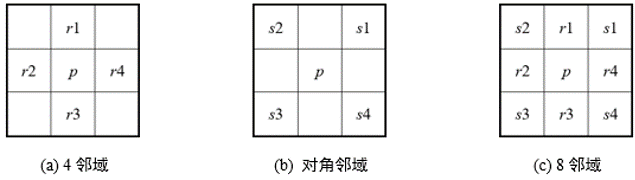
\includegraphics[width=0.6\textwidth]{邻域.png}
    \caption{邻域的类型}
\end{figure}

\subsubsection{像素的邻接}

一个像素与在它邻域中的像素是接触的,称为邻接。

和邻域类型相对应,像素邻接的类型包括:4邻接、对角邻接、8邻接。

\subsubsection{像素的连接}

像素的连接:邻接且灰度值(或其他属性)满足某个特定的相似准则(相等或在同一集合)。

像素连接的类型包括:4连接、8连接和$m$连接(混合连接)。

4连接:两个像素$p$和$r$在$V$中取值且$r$在$N_4(p)$中。

8连接:两个像素$p$和$r$在$V$中取值且$r$在$N_8(p)$中。

$m$-连接:两个像素$p$和$r$在$V$中取值且满足两个条件之一:

\textcircled{1} $r$在$N_4(p)$中(即$p$和$r$是4连接);

\textcircled{2} $r$在$N_D(p)$中且$N_4(p)∩N_4(r)$(即与$p$和$r$同时4邻接的两个像素)不包含$V$中取值的像素。

\subsubsection{像素的通路}

从具有坐标$(x, y)$的像素$p$到具有坐标$(s, t)$的像素$q$的一条通路由一系列具有坐标$(x_0, y_0)$,$(x_1, y_1)$,…,$(x_n, y_n)$的独立像素组成。

根据不同的邻接定义,可以得到不同的通路。

\subsubsection{像素的连通}

像素间通路上所有像素的灰度值均满足某个特定的相似准则,则像素$p$和$q$是连通的。

根据不同的连接定义,可以得到不同的连通。

连接可以看作是像素连通的一种特例。两个连通的像素也是连接的。

\subsubsection{像素集合的邻接}

对两个图像子集$S$和$T$来说,如果$S$中的一个或一些像素与$T$中的一个或一些像素邻接,则可以说两个图像子集$S$和$T$是邻接的。

\subsubsection{像素集合的连接}

对两个图像子集$S$和$T$来说,如果$S$中的一个或一些像素与$T$中的一个或一些像素连接,则可以说两个图像子集$S$和$T$是连接的。

\subsubsection{像素集合的连通}

设$p$和$q$是一个图像子集$S$中的两个像素,如果存在一条完全由在$S$中的像素组成的从$p$到$q$的通路,则称$p$在$S$中与$q$连通。

对$S$中任一个像素$p$,所有与$p$相连通且又在$S$中的像素的集合(包括$p$)合起来称为$S$中的一个连通组元。

\subsection{像素间的距离}

\subsubsection{欧式距离}

$D_E$距离,即欧氏距离,是范数为2的距离。点$p$和$q$之间的欧氏距离定义为:

\begin{equation}
    D_E(p,q)=\sqrt{(x_1-x_2)^2+(y_1-y_2)^2}
\end{equation}

\subsubsection{城区距离}

$D_4$距离,即城区距离,是范数为1的距离。点$p$和$q$之间的城区距离定义为:

\begin{equation}
    D_4(p,q)=|x_1-x_2|+|y_1-y_2|
\end{equation}

两点$p$和$q$之间的$D_4$距离等于它们之间最短的4通路的长度。

\subsubsection{棋盘距离}

$D_8$距离,即棋盘距离,是范数为$\infty$的距离。点$p$和$q$之间的城区棋盘定义为:

\begin{equation}
    D_8(p,q)=\max(|x_1-x_2|,|y_1-y_2|)
\end{equation}

两点$p$和$q$之间的$D_8$距离等于它们之间最短的8通路的长度。

\subsubsection{混合距离}

两个像素点$p$和$q$之间的混合距离$D_m(p,q)$等于它们之间满足混合连通的通路的长度。

\subsection{几何变换}

几何变换的本质是矩阵运算。设空间一个点的笛卡尔坐标为$(x,y,z)$,基于某个条件将其变换到新的坐标$(x',y',z')$,则几何变换公式可表示为矩阵形式:

\begin{equation}
    \bm{P'}=\left[
        \begin{array}{c}
            x' \\ y' \\ z' \\ 1
        \end{array}
    \right]=\left[
        \begin{array}{cccc}
            a_{11} & a_{12} & a_{13} & a_{14} \\
            a_{21} & a_{22} & a_{23} & a_{24} \\
            a_{31} & a_{32} & a_{33} & a_{34} \\
            a_{41} & a_{42} & a_{43} & a_{44}
        \end{array}
    \right]\left[
        \begin{array}{c}
            x \\ y \\ z \\ 1
        \end{array}
    \right]=\bm{AP}
\end{equation}

$\bm{P}=(x,y,z,1)^T$为点$(x,y,z)$对应的规范化齐次坐标;$\bm{P'}$为变换后的规范化齐次坐标;$\bm{A}$称为几何变换矩阵,唯一地确定几何变换的结果。

\subsubsection{平移变换}

\begin{equation}
    \bm{P'}=\left[
        \begin{array}{c}
            x' \\ y' \\ z' \\ 1
        \end{array}
    \right]=\left[
        \begin{array}{cccc}
            1 & 0 & 0 & a \\
            0 & 1 & 0 & b \\
            0 & 0 & 1 & c \\
            0 & 0 & 0 & 1
        \end{array}
    \right]\left[
        \begin{array}{c}
            x \\ y \\ z \\ 1
        \end{array}
    \right]=\bm{TP}=\left[
        \begin{array}{c}
            x+a \\ y+b \\ z+c \\ 1
        \end{array}
    \right]
\end{equation}

其中,$\bm{T}$为平移变换矩阵,$a,b,c$为平移系数,共同构成平移向量$(a,b,c)$。

\subsubsection{放缩变换}

\begin{equation}
    \bm{P'}=\left[
        \begin{array}{c}
            x' \\ y' \\ z' \\ 1
        \end{array}
    \right]=\left[
        \begin{array}{cccc}
            a & 0 & 0 & 0 \\
            0 & b & 0 & 0 \\
            0 & 0 & c & 0 \\
            0 & 0 & 0 & 1
        \end{array}
    \right]\left[
        \begin{array}{c}
            x \\ y \\ z \\ 1
        \end{array}
    \right]=\bm{SP}=\left[
        \begin{array}{c}
            ax \\ by \\ cz \\ 1
        \end{array}
    \right]
\end{equation}

其中,$\bm{S}$为放缩变换矩阵,$a,b,c$为放缩系数,共同构成放缩向量$(a,b,c)$。当$a=b=c$时,为尺度放缩,否则为拉伸放缩。

当放缩系数不为整数时,原始图像中某些像素放缩后的坐标可能不为整数,导致变换后的图像中出现“孔洞”现象,此时,需要经过取整或插值等操作来进行失真校正。

\subsubsection{旋转变换}

\textbf{2D平面的旋转}

\begin{equation}
    \left[
        \begin{array}{c}
            x' \\ y' 
        \end{array}
    \right]=\left[
        \begin{array}{cc}
            \cos{a}  & \sin{a} \\
            -\sin{a} & \cos{a} \\
        \end{array}
    \right]\left[
        \begin{array}{c}
            x \\ y 
        \end{array}
    \right]
\end{equation}

\textbf{绕$Z$坐标轴旋转}

\begin{equation}
    \bm{P'}=\left[
        \begin{array}{c}
            x' \\ y' \\ z' \\ 1
        \end{array}
    \right]=\left[
        \begin{array}{cccc}
            \cos{\gamma}  & \sin{\gamma} & 0 & 0 \\
            -\sin{\gamma} & \cos{\gamma} & 0 & 0 \\
            0 & 0 & 1 & 0 \\
            0 & 0 & 0 & 1
        \end{array}
    \right]\left[
        \begin{array}{c}
            x \\ y \\ z \\ 1
        \end{array}
    \right]=\bm{R_{\gamma}P}=\left[
        \begin{array}{c}
            x\cos{\gamma}+y\sin{\gamma} \\ 
            -x\sin{\gamma+y\cos{\gamma} \\
            z \\
            1
        \end{array}
    \right]
\end{equation}

\textbf{绕$Y$坐标轴旋转}

\begin{equation}
    \bm{P'}=\left[
        \begin{array}{c}
            x' \\ y' \\ z' \\ 1
        \end{array}
    \right]=\left[
        \begin{array}{cccc}
            \cos{\beta}  & 0 & \sin{\beta} & 0 \\
            0 & 1 & 0 & 0 \\
            -\sin{\beta} & 0 & \cos{\beta} & 0 \\
            0 & 0 & 0 & 1
        \end{array}
    \right]\left[
        \begin{array}{c}
            x \\ y \\ z \\ 1
        \end{array}
    \right]=\bm{R_{\beta}P}=\left[
        \begin{array}{c}
            x\cos{\beta}+z\sin{\beta} \\ 
            y \\
            -x\sin{\beta+z\cos{\beta} \\
            1
        \end{array}
    \right]
\end{equation}

\textbf{绕$X$坐标轴旋转}

\begin{equation}
    \bm{P'}=\left[
        \begin{array}{c}
            x' \\ y' \\ z' \\ 1
        \end{array}
    \right]=\left[
        \begin{array}{cccc}
            1  & 0 & 0 & 0 \\
            0 & \cos{\alpha}  & \sin{\alpha} & 0 \\
            0 & -\sin{\alpha} & \cos{\alpha} & 0 \\
            0 & 0 & 0 & 1
        \end{array}
    \right]\left[
        \begin{array}{c}
            x \\ y \\ z \\ 1
        \end{array}
    \right]=\bm{R_{\alpha}P}=\left[
        \begin{array}{c}
            x \\
            y\cos{\alpha}+z\sin{\alpha} \\ 
            -y\sin{\alpha+z\cos{\alpha} \\
            1
        \end{array}
    \right]
\end{equation}

\subsubsection{镜像变换}

\textbf{水平镜像}

\begin{equation}
    \bm{P'}=\left[
        \begin{array}{c}
            x' \\ y' \\ z' \\ 1
        \end{array}
    \right]=\left[
        \begin{array}{cccc}
            -1 & 0 & 0 & w \\
             0 & 1 & 0 & 0 \\
             0 & 0 & 1 & 0 \\
             0 & 0 & 0 & 1
        \end{array}
    \right]\left[
        \begin{array}{c}
            x \\ y \\ z \\ 1
        \end{array}
    \right]=\bm{M_{x}P}=\left[
        \begin{array}{c}
            -x+w \\ y \\ z \\ 1
        \end{array}
    \right]
\end{equation}

其中,$\bm{M_{x}}$为水平镜像变换矩阵,$w$为图像宽度。

\textbf{垂直镜像}

\begin{equation}
    \bm{P'}=\left[
        \begin{array}{c}
            x' \\ y' \\ z' \\ 1
        \end{array}
    \right]=\left[
        \begin{array}{cccc}
            1 &  0 & 0 & 0 \\
            0 & -1 & 0 & h \\
            0 &  0 & 1 & 0 \\
            0 &  0 & 0 & 1
        \end{array}
    \right]\left[
        \begin{array}{c}
            x \\ y \\ z \\ 1
        \end{array}
    \right]=\bm{M_{y}P}=\left[
        \begin{array}{c}
            x \\ -y+h \\ z \\ 1
        \end{array}
    \right]
\end{equation}

其中,$\bm{M_{y}}$为垂直镜像变换矩阵,$h$为图像高度。

\subsubsection{剪切变换}

\textbf{水平剪切}

\begin{equation}
    \bm{P'}=\left[
        \begin{array}{c}
            x' \\ y' \\ z' \\ 1
        \end{array}
    \right]=\left[
        \begin{array}{cccc}
            1 & 0 & 0 & 0 \\
            a & 1 & 0 & 0 \\
            0 & 0 & 1 & 0 \\
            0 & 0 & 0 & 1
        \end{array}
    \right]\left[
        \begin{array}{c}
            x \\ y \\ z \\ 1
        \end{array}
    \right]=\bm{H_{x}P}=\left[
        \begin{array}{c}
            x \\ ax+y \\ z \\ 1
        \end{array}
    \right]
\end{equation}

其中,$\bm{H_{x}}$为水平剪切变换矩阵,$a$为水平剪切系数。

\textbf{垂直剪切}

\begin{equation}
    \bm{P'}=\left[
        \begin{array}{c}
            x' \\ y' \\ z' \\ 1
        \end{array}
    \right]=\left[
        \begin{array}{cccc}
            1 & b & 0 & 0 \\
            0 & 1 & 0 & 0 \\
            0 & 0 & 1 & 0 \\
            0 & 0 & 0 & 1
        \end{array}
    \right]\left[
        \begin{array}{c}
            x \\ y \\ z \\ 1
        \end{array}
    \right]=\bm{H_{y}P}=\left[
        \begin{array}{c}
            x+by \\ y \\ z \\ 1
        \end{array}
    \right]
\end{equation}

其中,$\bm{H_{y}}$为垂直剪切变换矩阵,$b$为垂直剪切系数。

\subsubsection{透视变换}

\begin{equation}
    \bm{P'}=\left[
        \begin{array}{c}
            x' \\ y' \\ z' \\ 1
        \end{array}
    \right]=\left[
        \begin{array}{cccc}
            1 & 0 & 0 & 0 \\
            0 & 1 & 0 & 0 \\
            0 & 0 & 1 & 0 \\
            a & b & c & 1
        \end{array}
    \right]\left[
        \begin{array}{c}
            x \\ y \\ z \\ 1
        \end{array}
    \right]=\bm{EP}=\left[
        \begin{array}{c}
            x \\ y \\ z \\ ax+by+cz+1
        \end{array}
    \right]
\end{equation}

其中,$\bm{E}$为透视变换矩阵,$a,b,c$为透视变换系数,透视面为$ax+by+cz=0$。

\subsubsection{反变换}

平移变换、旋转变换和剪切变换的反变换为把对应的系数取负数。

放缩变换的反变换为把对应的系数取倒数。

镜像变换的反变换与正变换相同。

\subsubsection{复合变换}

多个几何变换复合成的变换,表示为:

\begin{equation}
    \bm{P'}=\bm{A_1 A_2 ... A_n P}=\bm{AP}
\end{equation}

其中$\bm{A_1,A_2,...,A_n}$为几个几何变换的变换矩阵,$\bm{A}$称为复合变换矩阵。

\subsection{几何失真校正}

几何失真是指图像在获取或显示过程中产生的畸变,也称几何畸变。如枕形失真、桶形失真、透视失真。

几何失真校正的校正方法包括直接法和间接法。校正步骤包括空间变换和灰度插值。

\subsubsection{直接校正法}

直接矫正法也称为向前映射法,由空间变换函数推导出反变换函数,然后计算畸变坐标对应的校正坐标;校正坐标一般不为整数,故将畸变图像像素的灰度值分配给校正坐标周围的四个像素,据此获得校正图像。

直接矫正法的不足:

\begin{enumerate}
    \item 畸变图像像素可能会被映射到校正图像之外,因此计算效率不高;
    \item 校正图像像素的灰度值由畸变图像像素的贡献之和决定,导致分配时存在较多的寻址,特别是在高阶插值时;
    \item 生成校正图像的像素分布不规则,容易出现像素挤压、疏密不均等现象,需要通过灰度插值方法生成规则的栅格图像。
\end{enumerate}

\subsubsection{间接校正法}

间接矫正法也称为向后映射法,由校正坐标计算出对应畸变坐标;畸变坐标一般不为整数,故将畸变坐标周围像素的灰度值进行插值以得到校正坐标处的灰度值,据此获得校正图像。

间接矫正法生成的校正图像由逐个像素通过一步插值得到,灰度插值效率较高,在实际应用中被广泛使用。

\subsubsection{空间变换}

空间变换是指对畸变图像像素坐标位置进行重新排列以恢复原始图像像素坐标位置的空间关系。

\subsubsection{灰度插值}

灰度插值是指对图像映射位置及其周围像素的灰度值进行插值操作以复原原始图像像素的灰度值。常用的灰度插值方法包括最近邻插值法、双线性插值法和双三次插值法等。

最近邻插值法:也称为零阶插值,将距离映射位置最近的像素点的灰度值作为插值结果。计算量小,但细微结构粗糙,容易出现块状效应。

双线性插值法:将映射位置周围四个像素点的灰度值在水平和垂直两个方向上进行插值以获取插值结果。具有低通滤波器的性质,它消弱了高频信息,导致图像轮廓模糊。

双三次插值法:将映射位置周围十六个像素点的灰度值在水平和垂直两个方向上进行插值以获取插值结果。计算精度高,较好地保持了图像的边缘细节,但计算量较大。

\section{空域图像增强}

图像增强是指将不清晰的图像变得清晰,强调某些关注的特征而抑制非关注的特征,以改善图像质量、丰富图像信息量、加强图像判读和识别效果的图像处理方法。图像增强包括空域图像增强和频域图像增强。

\begin{equation}
    \notag
    \text{空域图像增强}\left\{
        \begin{array}{l}
            \text{按图像的类型}\left\{
                \begin{array}{l}
                    \text{灰度增强} \\
                    \text{彩色增强}
                \end{array}
            \right. \\
            \text{按图像的范围}\left\{
                \begin{array}{l}
                    \text{局部增强} \\
                    \text{全局增强}
                \end{array}
            \right. \\
            \text{按像素的多少}\left\{
                \begin{array}{l}
                    \text{变换增强(点操作)}\left\{
                        \begin{array}{l}
                            \text{灰度操作} \\
                            \text{几何操作}
                        \end{array}
                    \right. \\
                    \text{滤波增强(模板操作)}
                \end{array}
            \right.
        \end{array}
    \right.
\end{equation}

空域变换增强也称为点操作,主要以单个像素为基础对图像进行增强。由于点可以看作是尺度为1×1的邻域,因此,点操作可以看作是模板操作的特例。

空域变换增强技术通常包括算术运算、逻辑运算、灰度变换和直方图处理。

\subsection{算术运算}

算术运算一般用于灰度图像,指将两个像素的灰度值通过算术操作得到一个新的灰度值,作为对应结果新图像同位置处像素的灰度值。

新的灰度值可能超出原图像的动态范围,此时,通常需要进行灰度映射。灰度映射将运算结果的灰度值限制或调整到原图像允许的动态范围内。

运算结果如果小于0,则取0;如果大于255,则取255。

\subsubsection{加法运算}

加法运算用于图像平均以减少和去除图像采集中混入的噪声。原始图像消噪前后均方差的关系为:

\begin{equation}
    \sigma_{\bar{g}(x,y)}=\sqrt{\frac{1}{M}}\sigma_{e(x,y)}
\end{equation}

其中$M$为样本图像的数量,$\sigma_{\bar{g}(x,y)}$为消噪后图像噪声的均方差,$\sigma_{e(x,y)$为消噪前图像噪声的均方差。

\subsubsection{减法运算}

减法运算可实现增强或减弱图像亮度以及运动检测等。

\subsubsection{乘法运算}

乘法运算可实现增强或减弱图像亮度以及图像掩模等。

\subsubsection{除法运算}

如果结果为小数,则要进行取整操作。如果分子分母均为0,则结果为0;如果仅分母为0,则结果为255。

对于灰度图像,白与白相除为黑;对于二值图像,白与白相除为白。

除法运算可实现增强或减弱图像亮度;校正成像设备的非线性影响;消除空间可变的量化敏感函数;对饱和度进行归一化;检测两幅图像间像素值的变化比率。除法运算也称为比率变换。

\subsection{逻辑运算}

逻辑运算包括与运算、或运算、补运算、异或运算。

进行逻辑运算时,将0作为假,非零作为真,运算结果为二值图像。

逻辑运算的典型应用为边缘检测。基于逻辑运算的边缘检测算法包括以下5个步骤:

\begin{enumerate}
    \item 设原始图像为图(a);
    \item 将图(a)的像素向左移动1个像素的位置得到图(b);
    \item 将图(a)和图(b)进行逻辑或运算得到图(c);
    \item 将图(a)和图(c)进行逻辑异或运算得到图(d);
    \item 对左右上下共4个方向(三维图像为6个方向)都进行上述操作得到4个结果图像,将4个结果图像进行逻辑或运算得到原图像的边缘。
\end{enumerate}

\begin{figure}[htbp]
    \centering
    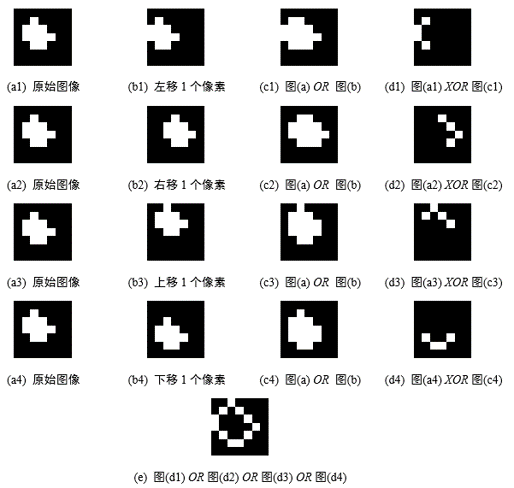
\includegraphics[width=0.6\textwidth]{边缘检测.png}
    \caption{基于逻辑运算的边缘检测}
\end{figure}

\subsection{直方图处理}

直方图处理属于空域变换增强技术。

图像的灰度级集中在较窄的区间,引起图像细节模糊时,可以用直方图变换对图像进行增强。直方图变换可以清晰图像细节,突出目标物体,改善亮度比例关系,增强图像对比度。

\subsubsection{直方图均衡化}

直方图均衡化借助灰度统计直方图和灰度累积直方图来进行。

灰度统计直方图反映了图像中不同灰度级出现的统计情况。灰度统计直方图是一个一维离散函数,可表示为:

\begin{equation}
    h(k)=n_k, \quad 0\leq k \leq L-1
\end{equation}

其中$k$为某个灰度级;$L$为灰度级的数量,最大取256;$n_k$为具有第$k$级灰度值的像素的数目。

\begin{figure}[htbp]
    \centering
    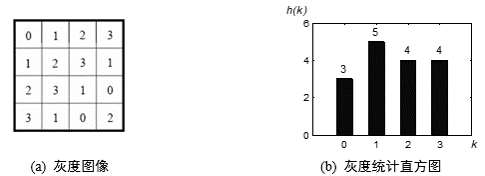
\includegraphics[width=0.5\textwidth]{灰度统计直方图.png}
    \caption{灰度统计直方图}
\end{figure}

灰度统计直方图写成归一化的概率表达形式为:

\begin{equation}
    p_s(s_k)=\frac{n_k}{N}, \quad 0\leq k \leq L-1
\end{equation}

其中$s_k$为第$k$级灰度值的归一化表达形式,$s_k=k/255\in[0,1]$,$N$为图像中像素的总数。

$s_k$和$p_s(s_k)$范围都为$[0,1]$,即变换前后图像的灰度值的动态范围一致。

灰度累积直方图反映了图像中灰度级小于或等于某值的像素的个数。灰度累积直方图是一个一维离散函数,可表示为:

\begin{equation}
    H(k)=\sum_{i=0}^{k}n_i, \quad 0\leq k \leq L-1
\end{equation}

其中$n_i$为具有第$i$级灰度值的像素的数目。

灰度累积直方图的归一化概率表达形式称为累积分布函数,能将$s$的分布转换为$t$的均匀分布,可表示为:

\begin{equation}
    t_k=E(s_k)=\sum_{i=0}^{k}\frac{n_i}{N}=\sum_{i=0}^{k}p_s(s_i), \quad 0\leq k \leq L-1
\end{equation}

直方图均衡化主要用于增强动态范围偏小的图像的反差。把原图像的直方图转换为均匀分布的形式,增加像素灰度值的动态范围,增强图像整体对比度。

直方图均衡化的步骤:

\begin{enumerate}
    \item 列出原始图像的灰度级$k$,$0\leq k \leq L-1$;
    \item 列出原始图像第$k$级灰度值的归一化表达形式$s_k$;
    \item 统计各灰度级的像素数目$n_k$;
    \item 计算原始直方图,即各灰度级的频数$p_s(s_k)$;
    \item 用累积分布函数计算累积直方图$E(s_k)$;
    \item 进行取整扩展,计算映射后输出图像的灰度级$t_k=\text{INT}((L-1)E(s_k)+0.5)/255$,$0\leq k \leq P-1$;
    \item 确定映射关系$s_k\rightarrow t_k$;
    \item 统计映射后各灰度级的像素数目$n_k$;
    \item 计算新直方图,即映射后各灰度级的频数$p_t(t_k)$。
\end{enumerate}

% 直方图均衡化列表计算:
% \begin{table}[htbp]
%     \centering
%     \caption{直方图均衡化计算列表}
%     \begin{tabular}{cccccccccc}
%         \hline
%         序号 & 运算 & \multicolumn{8}{cccccccc}{结果} \\
%         \hline
%         1 & $k$ & 0 & 1 & 2 & 3 & 4 & 5 & 6 & 7 \\
%         \hline
%     \end{tabular}
% \end{table}

直方图均衡化的优点:能够增强整个图像的对比度。

直方图均衡化的缺点:增强效果不易控制;均衡化图像的动态范围扩大;直方图有高峰时处理后对比度可能过分增强;导致出现伪轮廓。

\subsubsection{直方图规定化}

直方图规定化指通过灰度映射函数,将原灰度直方图改造成所希望的直方图,从而有选择地增强某个灰度值范围内的对比度,使图像灰度值的分布满足特定的要求。

单映射规则(SML):从小到大依次找到使下式最小的$k$和$l$,对于每组$k$和$l$,分别将$p_s(s_k)$对应映射到$p_t(t_l)$。简单直观,但有时会产生较大的取整误差。

\begin{equation}
    \left|\sum_{i=0}^{k}p_s(s_i)-\sum_{j=0}^{l}p_t(t_j)\right|, \quad 0\leq k \leq L-1, 0\leq l \leq M-1
\end{equation}

组映射规则(GML):一个整数函数$I(l)$,$0\leq l\leq N-1$,满足$0\leq I(0)\leq …\leq I(l)\leq …\leq I(N-1)\leq M-1$,确定能使下式达到最小的$I(l)$。若$l=0$,则将$i$从$0$到$I(0)$的$p_s(s_i)$对应到$p_t(t_0)$;若$l\geq 1$,则将$i$从$I(l-1)+1$到$I(l)$的$p_s(s_i)$对应到$p_t(t_j)$。具有较好地效果。

绘图计算:

SML:原始累积直方图中的每个点都映射到最接近的规定化累计直方图中的数值,即最短连线。

GML:规定化累计直方图中的每个点都映射到最接近的原始累积直方图中的数值,即最短连线。

\subsection{灰度变换}

灰度变换是一种点操作,根据原始图像中每个像素的灰度值,按照某种映射规则将其转化为另一灰度值。

灰度变换可有效改善图像的视觉效果。灰度变换的关键在于根据增强要求设计灰度映射规则,即设计灰度增强函数$E(k)$。

典型灰度变换函数包括:比例线性变换、分段线性变换、非线性变换。

\subsubsection{比例线性变换}

比例线性变换包括正比变换和反比变换。正比变换包括直接正比变换和截取式正比变换。

直接正比变换将一部分灰度范围映射到$[0,255]$;截取式正比变换将边缘压缩为一个灰度值。

反比变换即黑白反转。

\subsubsection{分段线性变换}

分段线性变换局部扩展亮度值范围,从而增强图像的对比度。包括对比拉伸和灰度切割。

对比拉伸的基本思想是扩展图像的动态范围,增强图像的对比度,是最简单的分段线性变换之一。对有用部分进行扩展,无用部分进行压缩。

灰度切割提高图像中特定灰度范围的亮度。为范围内的灰度指定一个较高值,其他灰度指定一个较低值或保持原有的灰度。

\subsubsection{非线性变换}

非线性变换主要利用非线性函数来突出目标区域,达到最大限度增强图像中有用信息的目的。非线性变换包括对数变换和幂次变换。

对数变换:扩展低亮度、压缩高亮度。

幂次变换:扩展低亮度、压缩高亮度;或扩展高亮度、压缩低亮度。由幂次系数决定。

\section{空域滤波增强}

空域滤波增强也称为模板操作,主要以像素邻域为基础对图像进行增强,增强函数$E()$定义在像素点$(x,y)$的某个邻域上。模板是指滤波器、核、掩模或窗口。邻域可以是任意形状,通常采用正方形或矩形阵列。

空域滤波增强的基本原理是利用图像与模板的卷积来进行。

基于卷积的空域滤波增强的步骤为:

\begin{enumerate}
    \item 将模板在原始图像中漫游,并将模板中心与原始图像中的某个像素重合;
    \item 将模板上的各系数与模板下对应像素的灰度值相乘,再将所有乘积相加;
    \item 将运算结果(模板的输出响应)赋值给变换图像中对应模板中心位置的像素。
\end{enumerate}

\subsection{卷积原理}

\subsubsection{一维离散卷积}

\begin{figure}[htbp]
    \centering
    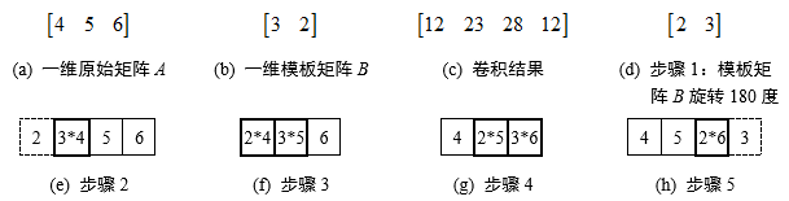
\includegraphics[width=0.6\textwidth]{一维离散卷积.png}
    \caption{一维离散卷积}
\end{figure}

\subsubsection{二维离散卷积}

卷积过程首先将模板矩阵旋转180度,然后从左到右、从上到下在原始矩阵中滑动,卷积结果中对应位置的数值等于模板矩阵与原始矩阵交集元素的乘积和。

\begin{figure}[htbp]
    \centering
    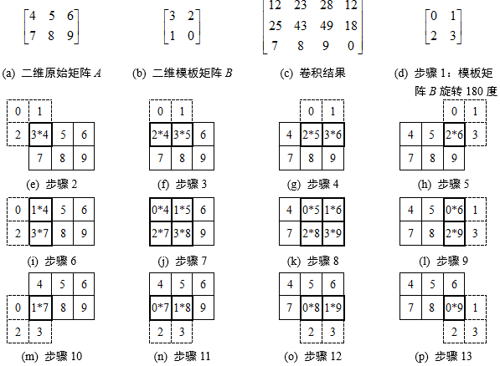
\includegraphics[width=0.6\textwidth]{二维离散卷积.png}
    \caption{二维离散卷积}
\end{figure}

\subsection{线性平滑滤波}

\subsubsection{邻域平均法}

典型模板:3$\times$3模板、8邻域模板、4邻域模板。

\begin{equation}
    \frac{1}{9}\left[
        \begin{array}{ccc}
            1 & 1 & 1 \\
            1 & 1 & 1 \\
            1 & 1 & 1
        \end{array}
    \right]\quad\quad
    \frac{1}{8}\left[
        \begin{array}{ccc}
            1 & 1 & 1 \\
            1 & 0 & 1 \\
            1 & 1 & 1
        \end{array}
    \right]\quad\quad
    \frac{1}{4}\left[
        \begin{array}{ccc}
            0 & 1 & 0 \\
            1 & 0 & 1 \\
            0 & 1 & 0
        \end{array}
    \right]
\end{equation}

经邻域平均法处理后,残余噪声的方差减小为原来的$1/k$,但引起原始图像中目标轮廓模糊或细节特征消失。

\subsubsection{选择平均法}

选择平均法以邻域平均法为基础,它只对灰度相同或相近的像素进行平均,或者按照灰度特殊的程度加权之后再求和,以免造成目标边缘的模糊。

常用的选择平均法:阀值法、半邻域法。

阀值法:当像素值与其邻域灰度均值之差较大时,必然是噪声,则取像素值为其邻域灰度均值;当像素值与其邻域灰度均值之差较小时,仍保留该像素的值。

半邻域法:设模板为3×3的矩阵。对$Ai$排序,灰度值较大的前5点构成$B$组,灰度值较小的后3点构成$A$组。设定门限阀值$T$并计算$A$、$B$两组的平均值$A_{avg}$和$B_{avg}$。若$|A_{avg}-B_{avg}\leq T|$,则认为无边缘通过,采用8邻域平均;反之,则认为有边缘通过,点$P$与$B$组中的5点进行6点平均。

\subsubsection{加权平均法}

离模板中心像素越近的像素对滤波结果的贡献越大,因此,可使接近模板中心的系数大些而模板边缘附件的系数小些。

高斯模板:

\begin{equation}
    \frac{1}{16}\left[
        \begin{array}{ccc}
            1 & 2 & 1 \\
            2 & 4 & 2 \\
            1 & 2 & 1
        \end{array}
    \right]
\end{equation}

\subsubsection{Wiener滤波}

Wiener滤波是一种在平稳条件下采用最小均方误差准则得出的最佳滤波准则。

\subsection{非线性平滑滤波}

\subsubsection{中值滤波}

把数字图像或图像序列中一点的值用该点的一个邻域中各点值的中值代替。既能消除噪声,又能保持图像细节。不适宜于一些细节多的图像。

较简单的模板是$n\times n$方形模板,$n$为奇数。若模板为$n\times n$,则输出值应大于等于模板中$(n^2-1)/2$个像素的值,小于等于模板中另$(n^2-1)/2$个像素的值。对于$3\times 3$的模板,中值是第5大的值。

\subsubsection{序统计滤波}

滤波原理基于模板所覆盖像素的灰度值的排序的滤波器。

常用的序统计滤波器包括:中值滤波器、最大值滤波器、最小值滤波器和中点滤波器。在计算卷积时不求和,而是按照以下规则选取所填入的值。

中值滤波器选取有序序列中位于50\%位置处的像素。

最大值滤波器选取有序序列中位于100\%位置处的像素。最大值滤波器用来检测图像中最亮的点并可减弱低取值的椒盐噪声。

最小值滤波器选取有序序列中位于0\%位置处的像素。最小值滤波器用来检测图像中最暗的点并可减弱高取值的椒盐噪声。

中点滤波器的输出为最大值和最小值中点的值。对多种随机分布的噪声(如高斯噪声、均匀噪声)都比较有效。

\subsection{线性锐化滤波}

一阶微分的差分定义:

\begin{equation}
    \frac{\partial f}{\partial x}=\frac{\mathrm{d}f}{\mathrm{d}x}=f(x+1)-f(x)
\end{equation}

二阶微分的差分定义:

\begin{equation}
    \frac{\partial^2 f}{\partial x^2}=f(x+1)+f(x-1)-2f(x)
\end{equation}

\subsection{非线性锐化滤波}

非线性锐化滤波技术基于非线性的微分方法。常用的非线性锐化滤波方法包括:梯度法、Prewitt算子、Sobel算子、Log算子、高通滤波、掩模法、Canny算子、Krisch算子等。

\section{图像变换}

\subsection{一维离散变换}



\subsection{二维离散变换}



\subsection{傅里叶变换}

\subsubsection{一维连续傅里叶变换}



\subsubsection{一维离散傅里叶变换}



\subsubsection{二维连续傅里叶变换}



\subsubsection{二维离散傅里叶变换}



\subsubsection{频域特征与空域特征的关系}



\subsubsection{傅里叶变换的应用}



\subsection{离散余弦变换}

\subsubsection{一维离散余弦变换}



\subsubsection{二维离散余弦变换}



\subsubsection{离散余弦变换的应用}



\section{频域图像增强}

\subsection{低通滤波}



\subsubsection{理想低通滤波器}



\subsubsection{巴特沃斯低通滤波器}



\subsubsection{指数低通滤波器}



\subsubsection{梯形低通滤波器}



\subsubsection{高斯低通滤波器}



\subsection{高通滤波}

\subsubsection{理想高通滤波器}



\subsubsection{巴特沃斯高通滤波器}



\subsubsection{指数高通滤波器}



\subsubsection{梯形高通滤波器}



\subsubsection{高斯高通滤波器}



\subsubsection{高频增强滤波器}



\subsection{频域增强与空域增强的关系}



\end{document}
